%TODO: Chapter needs to be improved a lot
\documentclass[11pt,compress,t,notes=noshow, aspectratio=169, xcolor=table]{beamer}

\usepackage{../../style/lmu-lecture}
% Defines macros and environments
% This file is included in slides and exercises

% Rarely used fontstyle for R packages, used only in 
% - forests/slides-forests-benchmark.tex
% - exercises/single-exercises/methods_l_1.Rnw
% - slides/cart/attic/slides_extra_trees.Rnw
\newcommand{\pkg}[1]{{\fontseries{b}\selectfont #1}}

% Spacing helpers, used often (mostly in exercises for \dlz)
\newcommand{\lz}{\vspace{0.5cm}} % vertical space (used often in slides)
\newcommand{\dlz}{\vspace{1cm}}  % double vertical space (used often in exercises, never in slides)
\newcommand{\oneliner}[1] % Oneliner for important statements, used e.g. in iml, algods
{\begin{block}{}\begin{center}\begin{Large}#1\end{Large}\end{center}\end{block}}

% Don't know if this is used or needed, remove?
% textcolor that works in mathmode
% https://tex.stackexchange.com/a/261480
% Used e.g. in forests/slides-forests-bagging.tex
% [...] \textcolor{blue}{\tfrac{1}{M}\sum^M_{m} [...]
% \makeatletter
% \renewcommand*{\@textcolor}[3]{%
%   \protect\leavevmode
%   \begingroup
%     \color#1{#2}#3%
%   \endgroup
% }
% \makeatother


\usepackage[export]{adjustbox}
\usepackage[most]{tcolorbox}

\newtcolorbox{BlueBox}[2][]{%
   enhanced,
   colback   = blue!5!white,
   colframe  = blue!65!black,
   arc       = 1mm,
   outer arc = 1mm,
   center title,
   title     = #2,
   #1}

\definecolor{winter}{RGB} {243,117,108}
\definecolor{spring}{RGB} {121,174,65}
\definecolor{summer}{RGB} {25,188,195}
\definecolor{fall}{RGB} {166,128,185}

\title{Interpretable Machine Learning}
% \author{LMU}
%\institute{\href{https://compstat-lmu.github.io/lecture_iml/}{compstat-lmu.github.io/lecture\_iml}}
\date{}

\begin{document}

\newcommand{\titlefigure}{figure/dependence_2}
\newcommand{\learninggoals}{
\item Pearson correlation
\item Coefficient of determination $R^2$
\item Mutual information
\item Correlation vs. dependence
}

\lecturechapter{Correlation and Dependencies}
\lecture{Interpretable Machine Learning}
%
% \begin{frame}{Interpretable ML}
% \begin{itemize}
% %\itemsep2em
% \item ML algorithms algorithmically train predictive models with no or little pre-specifications and assumptions about the data.
% \item Several algorithms such as decision tree learning create interpretable models. However, most algorithms create models which can be considered a black box.
% \item We use the term black box, although the internal workings of the model are in fact accessible, but too complex for the human mind to comprehend.
% \end{itemize}
% \end{frame}
%
% \begin{frame}{Explainable AI}
% \begin{itemize}
% %\itemsep1em
% \item IML is often used synonymously with Explainable AI (XAI).
% \item There is no unified standard for these terminologies. We find that XAI often is specifically concerned with the interpretation of neural networks, whereas IML is used as an encompassing term for everything related to model interpretability.
% \item The nature of (deep) neural networks allows for powerful model-specific interpretation techniques, e.g., layer-wise relevance propagation (LRP) and saliency maps.
% \item Also covering model-specific NN methods would exceed the timeframe of this lecture. This lecture will concentrate on model-agnostic techniques, as they are both versatile, and receive a lot of attention in industry and academia.
% \end{itemize}
% \end{frame}
%
% \begin{frame}{XAI - Saliency Maps}
%
% A saliency map is a heatmap indicating pixel influence on the prediction (e.g., a classification of an image): \footnote[frame]{Mundhenk, T., Chen, B.Y., Friedland, G. (2019). Efficient Saliency Maps for Explainable AI. ArXiv, abs/1911.11293.
% }
% \medskip
% \begin{figure}
% 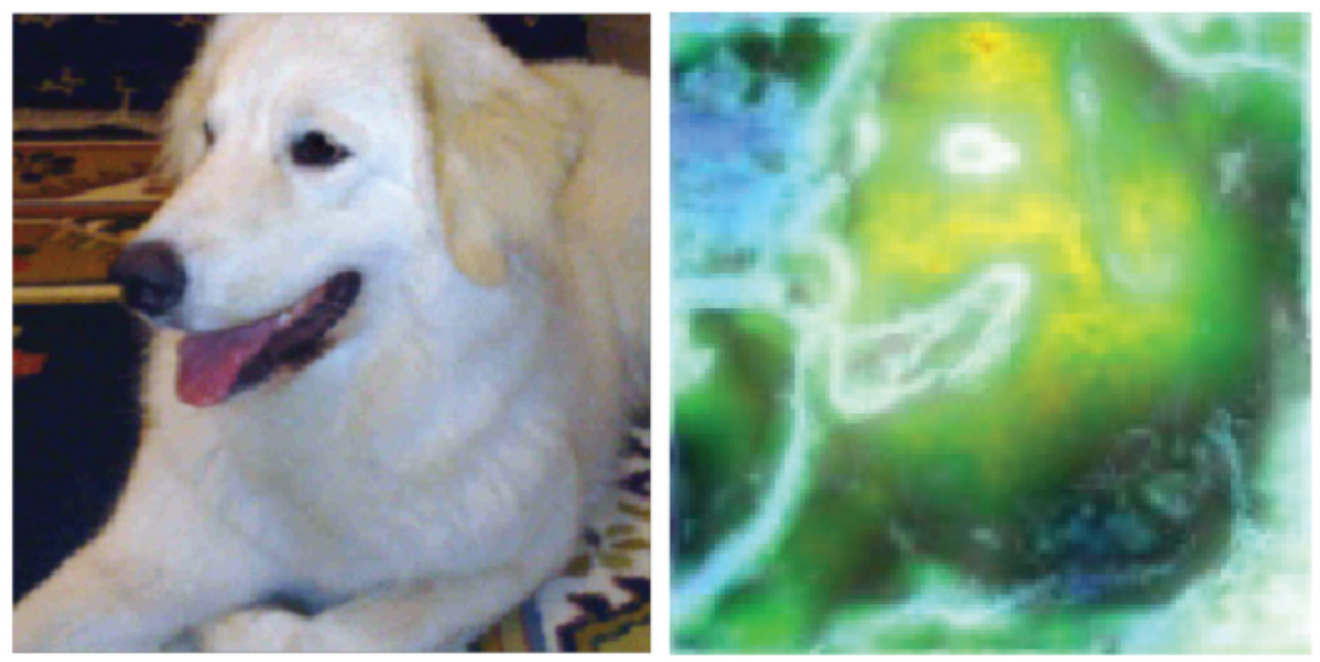
\includegraphics[width = 0.8 \textwidth]{figure/saliencymap}
% \end{figure}
% \end{frame}
%
% \begin{frame}{What is Interpretability?}
% \begin{itemize}
% %\itemsep1em
% \item There is no scientific consensus on the definition of interpretability.
% \item We need to differentiate between interpretations of a model or reality. The latter is distorted by all modeling fallacies involved in predictive modeling, e.g., data quality, under- and overfitting, or model extrapolations.
% \item We use a practical definition of interpretability.
% Think back to the foundations of statistical modeling:  the linear regression model (LM). The LM, with its known equation of beta coefficients, represents a paradigm for statistical interpretability.
% \item It follows that it would be beneficial to create techniques that give us an interpretation similar to the one of an LM.
%
% \end{itemize}
% \end{frame}


% \begin{frame}{Correlation and Dependence}
% \begin{itemize}
% \item \textbf{Correlation:} Often linear correlation (Pearson $\rho$) between pairs of features is meant
% \item \textbf{Dependence:} More general dependence structure (e.g., non-linear relationships)
% \item $X_j$, $X_k$ independent $\Leftrightarrow$ joint probability density function (PDF) is product of marginal PDFs:
% %$$\text{PDF}_{X_j, X_k}(x_j, x_k) = \text{PDF}_{X_j}(x_j) \cdot \text{PDF}_{X_k}(x_k)$$
% $$\P(X_j, X_k) = \P(X_j) \cdot \P(X_k)$$


% $\P(X_j|X_k) = \P(X_j)$ knowing $X_k$ does not tell us anything about $X_j$ and vice versa
% \item $X_j$, $X_k$ independent $\Rightarrow$ $X_j$, $X_k$ uncorrelated \textbf{but} $X_j$, $X_k$ uncorrelated $\nRightarrow$ $X_j$, $X_k$  independent
% %\item Auf einer slide eklären, visuell und mathematisch
% \end{itemize}

% \centering

% \only<1>{
% \textbf{Example:} $X_1$, $X_2 \sim N(0,1)$ independent ($\rho = 0$) \hspace{10pt} $X_1$, $X_2 \sim N(0,1)$ dependent ($\rho = 0.8$) \hspace{30pt}

% \includegraphics[width = 0.4\textwidth]{figure/independent}
% \includegraphics[width = 0.4\textwidth]{figure/dependent}
% }


% \only<2>{
% 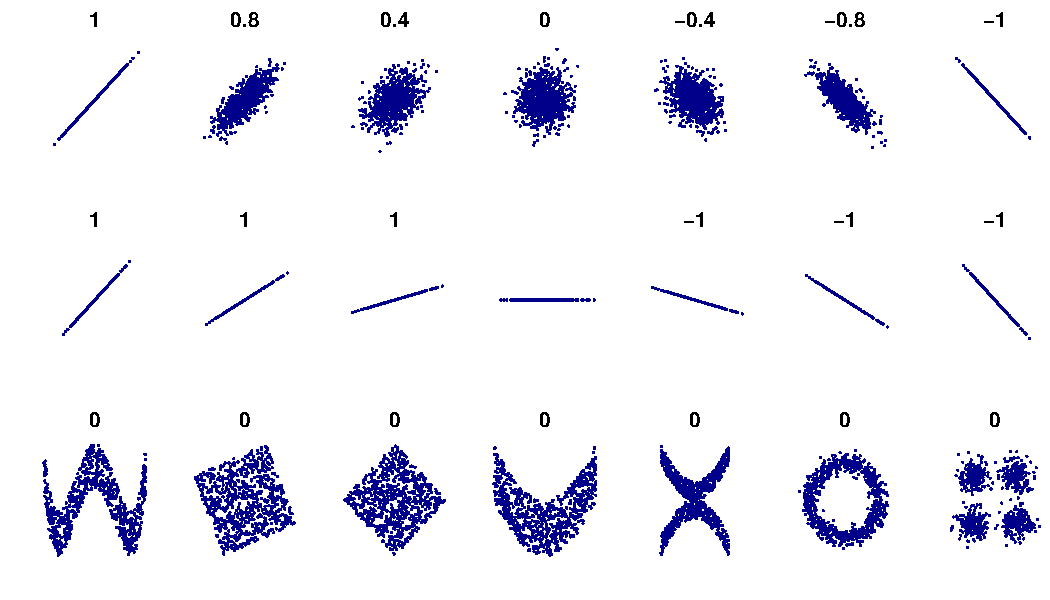
\includegraphics[width = 0.5\textwidth]{figure/dependence_2}
% }
% % correlation reflects the noisiness and direction of a linear relationship (top row), but not the slope of that relationship (middle), nor many aspects of nonlinear relationships (bottom). N.B.: the figure in the center has a slope of 0 but in that case the correlation coefficient is undefined because the variance of Y is zero.
% \end{frame}


\begin{frame}{Pearson's correlation coefficient $\rho$}

\textbf{Correlation} often refers to Pearson's correlation (measures only \textbf{linear relationship}) %between pairs of features
\smallskip

%\dfrac{s_{X_1 X_2}}{s_{X_1} \cdot s_{X_2}} \text{ with }

% \begin{itemize}
%     \item Sample covariance of $X_1$ and $X_2$:
%     $s_{X_1 X_2} = \frac{1}{n-1}\sum_{i=1}^{n}{(x_1^{(i)}-\bar{x}_1) \cdot (x_2^{(i)}-\bar{x}_2)}$
%     \item Sample standard deviation $s_{X_1}$ and $s_{X_2}$ of $X_1$ and $X_2$
% \end{itemize}

\centerline{$\rho(X_1, X_2) = \tfrac{\sum_{i=1}^{n}{(x_1^{(i)}-\bar{x}_1) \cdot (x_2^{(i)}-\bar{x}_2)}}{\sqrt{\sum_{i=1}^{n}{(x_1^{(i)}-\bar{x}_1)^2 \sum_{i=1}^{n}{(x_2^{(i)}-\bar{x}_2)^2 }}}} \in [-1, 1]$}

\bigskip

\begin{columns}[T, totalwidth=\textwidth]
\begin{column}{0.6\linewidth}
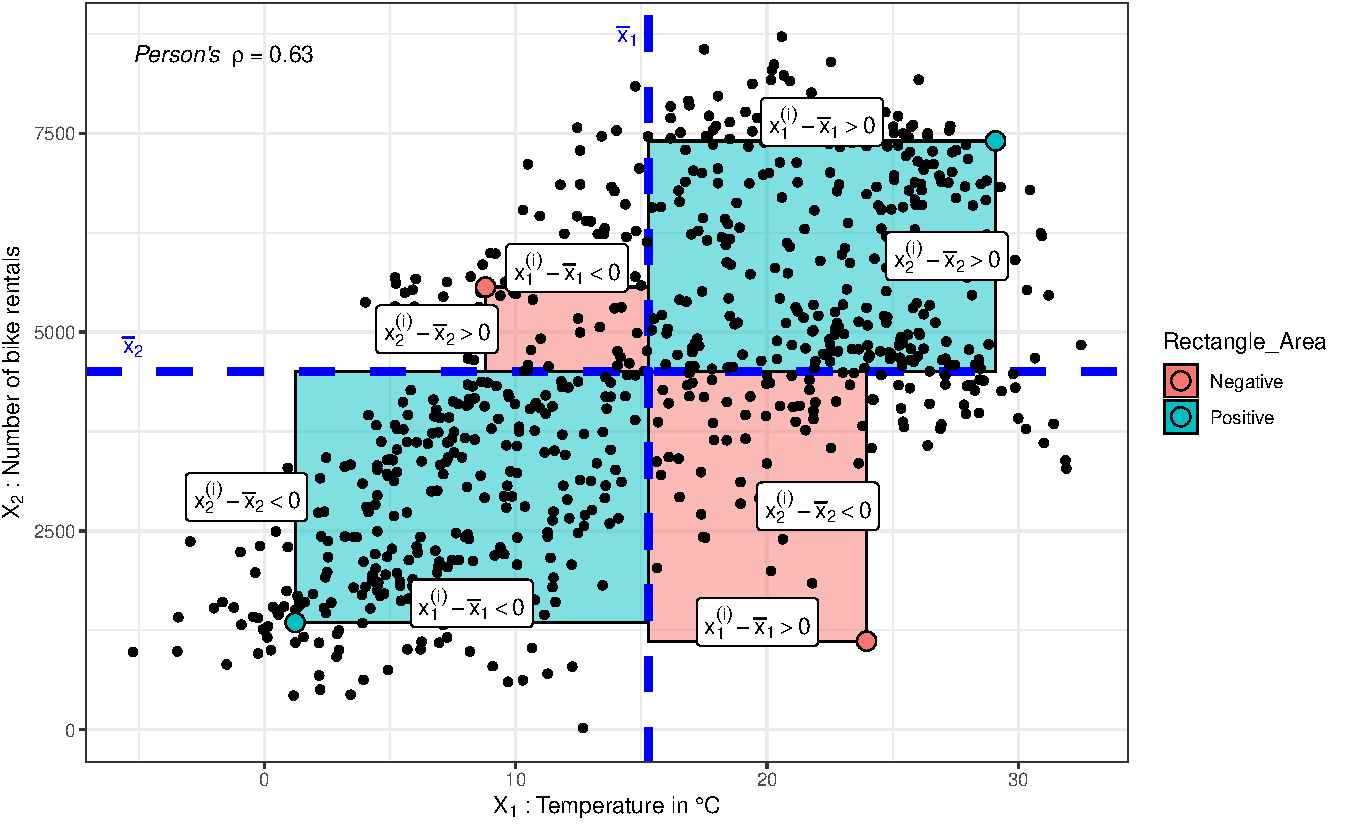
\includegraphics[width = \textwidth]{figure/pearson_cor}
\end{column}
\begin{column}{0.4\linewidth}

Geometric interpretation of $\rho$:
\begin{itemize}
    \item Numerator is sum of rectangle's area with width $x_1^{(i)}-\bar{x}_1$ and height $x_2^{(i)}-\bar{x}_2$
    \item Areas enter numerator with positive (\textbf{+}) or negative (\textbf{-}) sign, depending on position
    \item Denominator scales the sum into the range $[-1, 1]$
    %\item $\rho = 0$ if area of all rectangles cancels out\\
    %$\leadsto$ $X_1, X_2$ uncorrelated
\end{itemize}
\end{column}
\end{columns}

\medskip
\pause
\begin{itemize}
    \item $\rho > 0$ if {\color{ggblue}positive areas} dominate {\color{ggred}negative areas} 
    $\leadsto$ $X_1, X_2$ positive correlated
    \item $\rho < 0$ if {\color{ggred}negative areas} dominate {\color{ggblue}positive areas} 
    $\leadsto$ $X_1, X_2$ negative correlated
    \item $\rho = 0$ if area of rectangles cancels out
    $\leadsto$ $X_1, X_2$ linearly uncorrelated
\end{itemize}
%\textbf{But:} Pearson's $\rho$ does not measure non-linear dependencies, e.g., $\rho = 0$ but dependent:

\end{frame}


\begin{frame}{Coefficient of determination $R^2$}

Another method to evaluate \textbf{linear dependency} between features is $R^2$

\begin{columns}[c, totalwidth=\textwidth]
\begin{column}{0.52\linewidth}
\only<1>{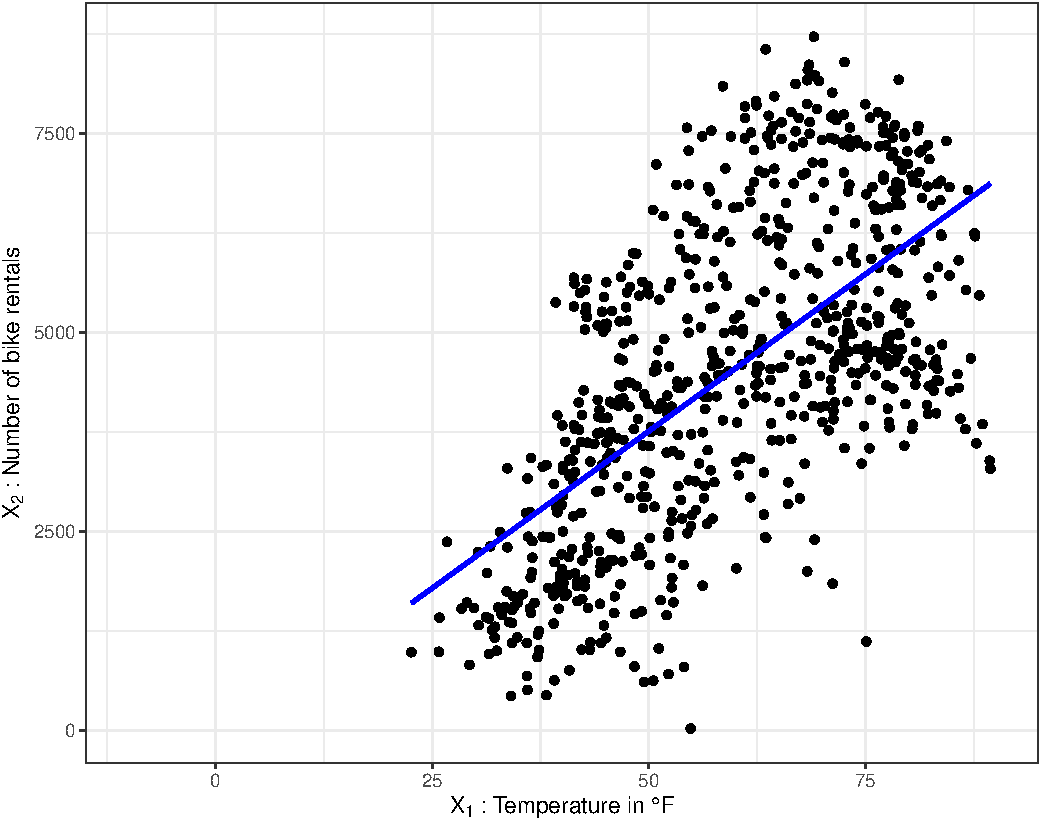
\includegraphics[width = \textwidth]{figure/r_squared_Fahrenheit}}
\only<2>{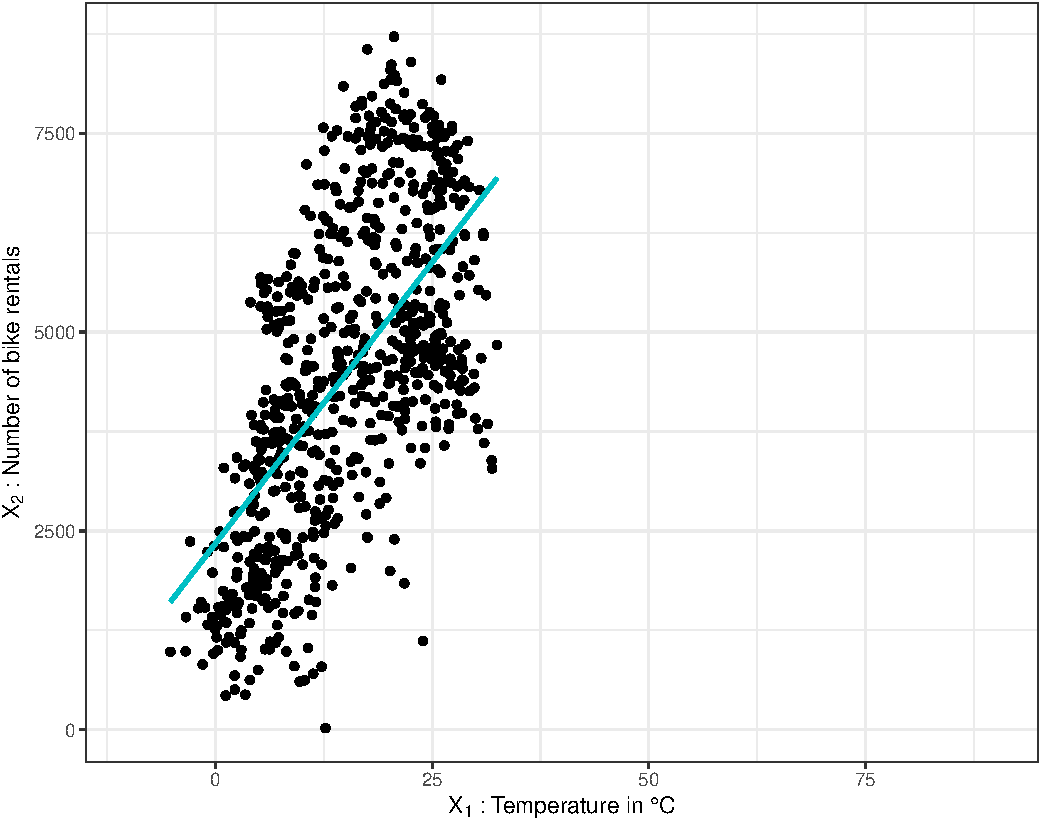
\includegraphics[width = \textwidth]{figure/r_squared_compare}}
\only<3>{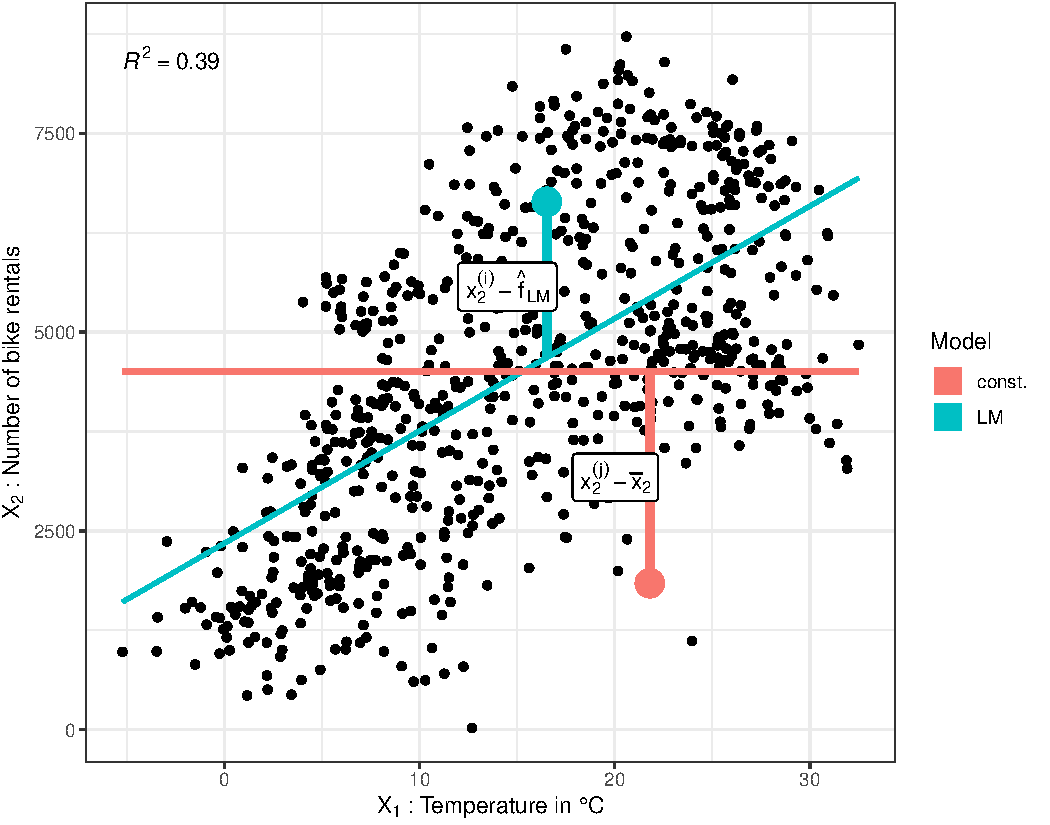
\includegraphics[width = \textwidth]{figure/r_squared}}
\end{column}
\begin{column}{0.48\linewidth}

\medskip

%Idea for two-dimensional case:
\begin{itemize}
    \setlength\itemsep{0.7mm}
    \item Fit a linear model:
    $\hat{x}_2 = \hat{f}_{LM}(x_1) = \theta_0 + \theta_1 x_1$
    %($x_2 \sim x_1$) 
    % $\hat{f}_{LM}(x_1) = 2345 + 141.3 x_1$
    \item[$\leadsto$] Slope $\theta_1$ = $0$ $\Rightarrow$ no dependence
    \item[$\leadsto$] Large slope $\Rightarrow$ strong dependence
        \pause
    \item Exact $\theta_1$ score problematic 
    \item[$\leadsto$] Re-scaling of $x_1$ or $x_2$ changes $\theta_1$ 
    \only<2>{\item[$\leadsto$] °F $\rightarrow$ °C $\Rightarrow$ ${\color{blue}\theta_1=78}\rightarrow{\color{ggblue}\theta_1^*=141}$}
    \pause
    \item Set $SSE_{LM}$ in relation to $SSE$ of a constant model $\hat{f}_c = \bar{x}_2$
    \item[] $SSE_{LM} = \sum_{i=1}^n ({\color{ggblue}x_2^{(i)} - \hat{f}_{LM}(x_1^{(i)})})^2$
    \item[] $SSE_{c} = \sum_{i=1}^n ({\color{ggred}x_2^{(i)} - \bar{x}_2})^2$
\end{itemize}

\end{column}
\end{columns}

\medskip

$\Rightarrow$ Measure of fitting quality of LM: $R^2 = 1-\frac{SSE_{LM}}{SSE_{c}} \in [0, 1]$ \\
$\Rightarrow \rho(X_1, X_2) = R$

\end{frame}


\begin{frame}{Joint, Marginal and Conditional Distribution}
    For two discrete random variables $X_1, X_2$:
    
    \begin{columns}[c, totalwidth=\textwidth]
    \begin{column}{0.5\textwidth}
    \textbf{Joint distribution}
        \begin{align*}
            p_{X_1, X_2}(x_1,x_2) = \P(X_1 = x_1, X_2 = x_2) %
        \end{align*}
    \end{column}
    \begin{column}{0.5\textwidth}
    \begin{table}
    \scriptsize
        %\vspace{-0.3cm}
        \begin{tabular}{|c|c|c|c|}
            \hline 
            $p_{X_1, X_2}$ & $\P(X_2 = 0)$ & $\P(X_2 = 1)$ & $p_{X_1}$ \\
            \hline
            $\P(X_1 = 0)$ & \cellcolor{gray}0.2 & \cellcolor{gray}0.3 & 0.5  \\
            \hline
            $\P(X_1 = 1)$ & \cellcolor{gray}0.1 & \cellcolor{gray}0.4 & 0.5  \\
            \hline
            $p_{X_2}$ & 0.3 & 0.7 & 1  \\
            \hline
        \end{tabular} 
    \end{table}
    \end{column}
    \end{columns} 

\medskip\pause
    
\begin{columns}[c, totalwidth=\textwidth]
    \begin{column}{0.5\textwidth}
    \textbf{Marginal distribution}
        \begin{align*}
            p_{X_1}(x_1) = \P(X_1 = x_1) = \sum_{x_2\in \mathcal{X}_2} p(x_1,x_2)
        \end{align*}    
        $\leadsto$ In continuous case with integrals
    \end{column}
    \begin{column}{0.5\textwidth}
    \begin{table}
    \scriptsize
        \begin{tabular}{|c|c|c|c|}
            \hline 
            $p_{X_1, X_2}$ & $\P(X_2 = 0)$ & $\P(X_2 = 1)$ & $p_{X_1}$ \\
            \hline
            $\P(X_1 = 0)$ & 0.2 & 0.3 & \cellcolor{gray}0.5  \\
            \hline
            $\P(X_1 = 1)$ & 0.1 & 0.4 & \cellcolor{gray}0.5  \\
            \hline
            $p_{X_2}$ & 0.3 & 0.7 & 1  \\
            \hline
        \end{tabular}
    \end{table}
    \end{column}
    \end{columns} 

    \medskip\pause
    
\begin{columns}[c, totalwidth=\textwidth]
    \begin{column}{0.5\textwidth}
    \textbf{Conditional distribution}
        \begin{align*}
            p_{X_1|X_2}(x_1 | x_2) &= \P(X_1=x_1| X_2 = x_2) \\&= \frac{p_{X_1, X_2}(x_1,x_2)}{p_{X_2}(x_2)}
        \end{align*}
 
    \end{column}
    \begin{column}{0.5\textwidth}
    \begin{table}
    \scriptsize
        \begin{tabular}{|c|c|c|c|}
            \hline 
             & $x_2 = 0$ & $x_2 = 1$ \\
            \hline
            $\P(X_1 = 0|X_2 =x_2)$ & \cellcolor{gray} 0.67 & \cellcolor{gray}0.43   \\
            \hline
            $\P(X_1 = 1|X_2 =x_2)$ & \cellcolor{gray} 0.33 & \cellcolor{gray}0.57   \\
            \hline
            $\sum$ & 1 & 1  \\
            \hline
        \end{tabular}
    \end{table}
    \end{column}
    \end{columns} 
\end{frame}



\begin{frame}{Dependence}
\textbf{Dependence:} Describes general dependence structure  (e.g., non-lin. relationships)

%\textbf{Definition:}
\begin{itemize}[<+->]
\item Definition: $X_j$, $X_k$ independent $\Leftrightarrow$ joint distribution is product of marginals:%\\ \vspace{5pt}
$$\P(X_j, X_k) = \P(X_j) \cdot \P(X_k)$$
%\vspace{5pt}
\item Equivalent definition (knowledge of $X_k$ says nothing about $X_j$ and vice versa): 
%\vspace{5pt}
$$\P(X_j|X_k) = \P(X_j) \text{ and } \P(X_k|X_j) = \P(X_k) \text{ (follows from cond. probability)}$$ 
%\vspace{5pt}
%$$\P(X_j|X_k) = \P(X_j) \hfill \text{(knowing $X_k$ does not tell us anything about $X_j$ and vice versa)}$$
%\medskip
\item Measuring complex dependencies is difficult but different measures exist, e.g., \\
$\leadsto$ Spearman correlation (measures monotonic dependencies via ranks) \\
$\leadsto$ Information-theoretical measures like mutual information \\
$\leadsto$ Kernel-based measures like Hilbert-Schmidt Independence Criterion (HSIC)
% nice further reading https://jejjohnson.github.io/research_journal/appendix/similarity/hsic/
\item \textbf{N.B.:} $X_j$, $X_k$ independent $\Rightarrow$ $\rho(X_j, X_k) = 0$ \textbf{but} $\rho(X_j, X_k) = 0$ $\nRightarrow$ $X_j$, $X_k$  indep. \\
Equivalency holds if distribution is jointly normal
\end{itemize}
\end{frame}


\begin{frame}{Mutual Information}
    \begin{itemize}
        \item MI describes expected amount of information shared by two random variables:% or how different the joint distribution is from pure independence
        $$MI(X_1, X_2 ) =  \mathbb{E}_{p(x_1, x_2)} \left[ log\left(\frac{p(x_1, x_2)}{p(x_1) p(x_2)} \right) \right] $$
        % \item $MI(X_1 ; X_2 )$ is the Kullback-Leibler distance between joint distribution $p(x_1, x_2)$ and the product of their marginal distribution $p(x_1) p(x_2)$:
        % \begin{align*}
        %     MI(X_1 ; X_2 ) &= \sum_{x_1 \in \mathcal{X}_1} \sum_{x_2 \in \mathcal{X}_2} p(x_1, x_2) log\left(\frac{p(x_1, x_2)}{p(x_1) p(x_2)} \right) \\
        %     &= D_{KL} \left( p(x_1, x_2) \, || \, p(x_1) p(x_2) \right) \\
        %     &= \mathbb{E}_{p(x_1, x_2)} \left[ log\left(\frac{p(x_1, x_2)}{p(x_1) p(x_2)} \right) \right]
        % \end{align*}
        \item MI measures amount of "dependence" between features by looking how different the joint distribution is from pure independence $p(x_1, x_2) = p(x_1) p(x_2)$\\
        $\leadsto$ $MI(X_1, X_2) = \mathbb{E}_{p(x_1, x_2)} \left[ log\left(\frac{p(x_1, x_2)}{p(x_1, x_2)} \right) \right] = \mathbb{E}_{p(x_1, x_2)} \left[ log(1) \right] = 0$\\
        $\leadsto$  $MI(X_j, X_k) = 0$ if and only if the features are independent
        \item Unlike (Pearson) correlation, MI can also be computed for categorical features %\\
        %$\leadsto$ Discrete RV: joint and marginal distribution obtained from confusion matrix\\
        %$\leadsto$ Continuous RV: Density estimation required, e.g., create bins via histogram
        %\item  $MI(X_j, X_k) = 0$ if and only if $X_j$, $X_k$ independent
    \end{itemize}
\end{frame}


% \begin{frame}{Mutual information: example 1}
% \begin{columns}[c, totalwidth=\textwidth]
%     \begin{column}{0.26\linewidth}
%         \begin{table}
%         \scriptsize
%         %\vspace{-0.3cm}
%         \begin{tabular}{|c|c|c|}
%             \hline 
%             $\bold{X}_1$ & ... & $\bold{Y}$ \\
%             \hline
%             yes & ... & yes  \\
%             yes & ... & yes  \\
%             yes & ... & yes  \\
%             yes & ... & no  \\
%             yes & ... & no  \\
%             no & ... & no  \\
%             \hline
%         \end{tabular} 
%         \end{table}

%     \end{column}
%     \begin{column}{0.74\linewidth}
%     \only<1>{
%     \scriptsize
%     \begin{table}
%     \begin{tabular}{|c|c|c|c|}
%         \hline 
%         & $\P(X_1 = \text{ yes})$ & $\P(X_1 = \text{ no})$ & $p_Y$ \\
%         \hline
%         $\P(Y = \text{ yes})$ & 0.5 & 0 & 0.5  \\
%         $\P(Y = \text{ no}) $& 0.333 & 0.167 & 0.5  \\
%         \hline
%         $p_{X_1}$ & 0.833 & 0.167 & 1 \\
%         \hline
%     \end{tabular} 
%     \end{table}}

%     \only<2-3>{
%     \scriptsize
%     \begin{table}
%     \begin{tabular}{|c|c|c|c|}
%         \hline 
%         & $\P(X_1 = \text{ yes})$ & $\P(X_1 = \text{ no})$ & $p_Y$ \\
%         \hline
%         $\P(Y = \text{ yes})$ & \cellcolor{summer}0.5 & \cellcolor{summer}0 & \cellcolor{spring}0.5  \\
%         $\P(Y = \text{ no}) $& \cellcolor{summer}0.333 & \cellcolor{summer}0.167 & \cellcolor{spring}0.5  \\
%         \hline
%         $p_{X_1}$ & \cellcolor{fall}0.833 & \cellcolor{fall}0.167 & 1 \\
%         \hline
%     \end{tabular} 
%     \end{table}}
        
%     \end{column}
% \end{columns}

% \only<2>{
% \vspace{-0.2cm}
% \begin{align*}
%             MI(X_1 ; Y) &= \sum_{x_1 \in \mathcal{X}_1} \sum_{y \in \mathcal{Y}} \textcolor{summer}{p(x_1, y)} log\left(\frac{\textcolor{summer}{p(x_1, y)}}{\textcolor{fall}{p(x_1)} \textcolor{spring}{p(y)}} \right) \\
%             &= \textcolor{summer}{\P(X_1 = \text{ yes}, Y = \text{ yes})}\, log\left(\frac{\textcolor{summer}{\P(X_1 = \text{ yes}, Y = \text{ yes})}}{\textcolor{fall}{\P(X_1 = \text{ yes})} \textcolor{spring}{\P(Y = \text{ yes})}} \right) \\
%             &\, + \textcolor{summer}{\P(X_1 = \text{ yes}, Y = \text{ no})}\, log\left(\frac{\textcolor{summer}{\P(X_1 = \text{ yes}, Y = \text{ no})}}{\textcolor{fall}{\P(X_1 = \text{ yes})} \textcolor{spring}{\P(Y = \text{ no})}} \right) \\
%             &\, + \textcolor{summer}{\P(X_1 = \text{ no}, Y = \text{ yes})}\, log\left(\frac{\textcolor{summer}{\P(X_1 = \text{ no}, Y = \text{ yes})}}{\textcolor{fall}{\P(X_1 = \text{ no})} \textcolor{spring}{\P(Y = \text{ yes})}} \right) \\
%             &\, + \textcolor{summer}{\P(X_1 = \text{ no}, Y = \text{ no})}\, log\left(\frac{\textcolor{summer}{\P(X_1 = \text{ no}, Y = \text{ no})}}{\textcolor{fall}{\P(X_1 = \text{ no})} \textcolor{spring}{\P(Y = \text{ no})}} \right) 
%         \end{align*}}
% \only<3>{
% \begin{align*}
%     MI(X_1 ; Y) = & \,\textcolor{summer}{0.5}\, log\left(\frac{\textcolor{summer}{0.5}}{\textcolor{fall}{0.833} \cdot \textcolor{spring}{0.5}} \right) 
%     + \textcolor{summer}{0.333}\, log\left(\frac{\textcolor{fall}{0.833}}{ \cdot \textcolor{spring}{0.5}} \right) \\
%     &+ \textcolor{summer}{0}\, log\left(\frac{\textcolor{summer}{0}}{\textcolor{fall}{0.167} \cdot \textcolor{spring}{0.5}} \right) 
%     + \textcolor{summer}{0.167}\, log\left(\frac{\textcolor{summer}{0.167}}{\textcolor{fall}{0.167} \cdot \textcolor{spring}{0.5}} \right) \\
%     = & \,0.133 \\
%     &\quad \\
%     \text{Note: } &lim_{x\rightarrow 0} \, x \, log\left(\frac{x}{c}\right) = 0, \, c \in \mathbb{R}
% \end{align*}

% }

% \end{frame}


\begin{frame}{Mutual information: example}
For two discrete RV $X_1$ and $Y$:
$$MI(X_1 ; Y ) =  \mathbb{E}_{p(x_1, y)} \left[ log\left(\frac{p(x_1, y)}{p(x_1) p(y)} \right) \right] = \sum_{x_1 \in \mathcal{X}_1} \sum_{y \in \mathcal{Y}} p(x_1, y) log\left(\frac{p(x_1, y)}{p(x_1) p(y)} \right) $$
\begin{columns}[c, totalwidth=\textwidth]
    \begin{column}{0.26\linewidth}
        \begin{table}
        \scriptsize
        %\vspace{-0.3cm}
        \begin{tabular}{|c|c|c|}
            \hline 
            $\Xv_1$ & ... & $\Yv$ \\
            \hline
            yes & ... & yes  \\
            yes & ... & no  \\
            no & ... & yes  \\
            no & ... & no  \\
            \hline
        \end{tabular} 
        \end{table}

    \end{column}
    \begin{column}{0.74\linewidth}
    \only<1>{
    \scriptsize
    \begin{table}
    \begin{tabular}{|c|c|c|c|}
        \hline 
        & $\P(X_1 = \text{ yes})$ & $\P(X_1 = \text{ no})$ & $p_Y$ \\
        \hline
        $\P(Y = \text{ yes})$ & 0.25 & 0.25 & 0.5  \\
        $\P(Y = \text{ no}) $& 0.25 & 0.25 & 0.5  \\
        \hline
        $p_{X_1}$ & 0.5 & 0.5 & 1 \\
        \hline
    \end{tabular} 
    \end{table}}

    \only<2>{
    \scriptsize
    \begin{table}
    \begin{tabular}{|c|c|c|c|}
        \hline 
        & $\P(X_1 = \text{ yes})$ & $\P(X_1 = \text{ no})$ & $p_Y$ \\
        \hline
        $\P(Y = \text{ yes})$ & \cellcolor{summer}0.25 & \cellcolor{summer}0.25 & \cellcolor{spring}0.5  \\
        $\P(Y = \text{ no}) $& \cellcolor{summer}0.25 & \cellcolor{summer}0.25 & \cellcolor{spring}0.5  \\
        \hline
        $p_{X_1}$ & \cellcolor{fall}0.5 & \cellcolor{fall}0.5 & 1 \\
        \hline
    \end{tabular} 
    \end{table}}
        
    \end{column}
\end{columns}

\only<2>{
\begin{align*}
    MI(X_1 ; Y) = & \,\textcolor{summer}{0.25}\, log\left(\frac{\textcolor{summer}{0.25}}{\textcolor{fall}{0.5} \cdot \textcolor{spring}{0.5}} \right) 
    + \textcolor{summer}{0.25}\, log\left(\frac{\textcolor{summer}{0.25}}{\textcolor{fall}{0.5} \cdot \textcolor{spring}{0.5}} \right) \\
    &+ \textcolor{summer}{0.25}\, log\left(\frac{\textcolor{summer}{0.25}}{\textcolor{fall}{0.5} \cdot \textcolor{spring}{0.5}} \right)
    +\textcolor{summer}{0.25}\, log\left(\frac{\textcolor{summer}{0.25}}{\textcolor{fall}{0.5} \cdot \textcolor{spring}{0.5}} \right)\\
    = & \,0.25\, log\left(\frac{0.25}{0.25} \right) \cdot 4 \\
    = & \,0.25\, log\left(1 \right) \cdot 4 = \,0
\end{align*}}


\end{frame}



\begin{frame}{Dependence and Independence}
	
\textbf{Example:}
\begin{columns}[T, totalwidth=\linewidth]
\begin{column}{0.49\linewidth}
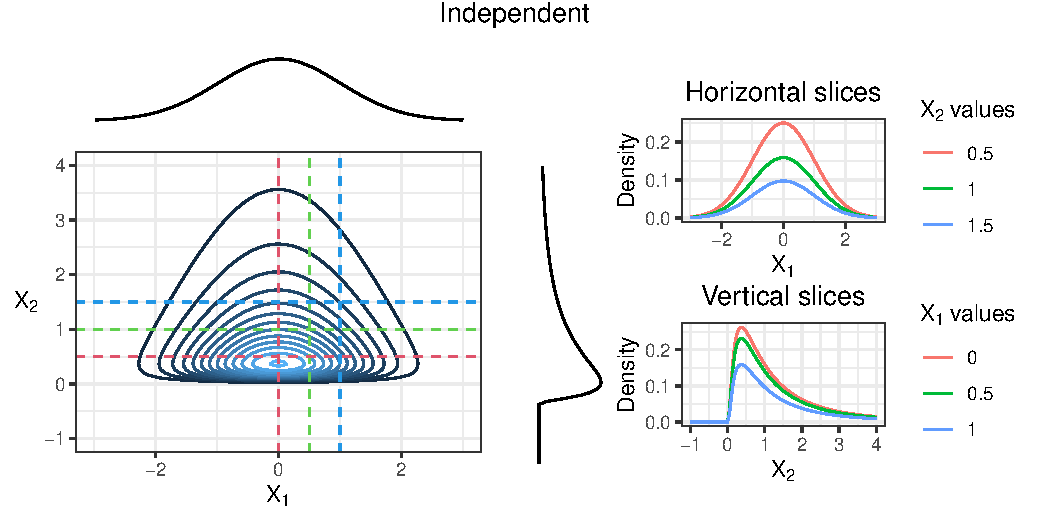
\includegraphics[width=\linewidth]{figure/independent_slice.pdf}
Conditional distributions at different vertical and horizontal slices (after normalizing area to 1) match their marginal distributions
% \begin{columns}[T, totalwidth=\linewidth]
% \begin{column}{0.6\linewidth}
% \vspace{-0.2cm}
\begin{align*}
    \Rightarrow \P(X_1|X_2) &= \P(X_1) \hspace{2.5cm} \\ 
    \P(X_2|X_1) &= \P(X_2)
\end{align*}
% \end{column}
% \begin{column}{0.4\linewidth}
% \end{column}
% \end{columns}
\end{column}
\hfill\pause
\begin{column}{0.49\linewidth}
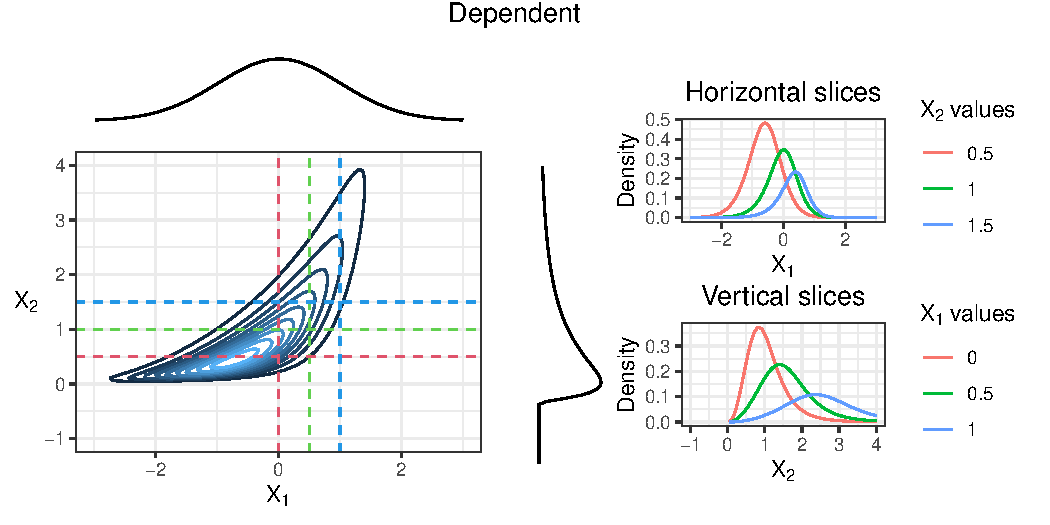
\includegraphics[width=\linewidth]{figure/dependent_slice.pdf}
Conditional distributions do not match their marginal distributions
\end{column}
\end{columns}


\end{frame}



\begin{frame}{Correlation vs. Dependence}

%Scatterplot with multivariate distribution (contour lines) and marginal density\\ 
Illustration of bivariate normal distribution with different correlations
$X_1$, $X_2 \sim N(0,1)$ 

\only<1>{\begin{center}
\begin{minipage}[t]{0.3\textwidth}
\centering
 $\rho(X_1, X_2) = 0$ \\(independent)
\end{minipage}
\begin{minipage}[t]{0.3\textwidth}
\centering
 $\rho(X_1, X_2) = 0.8$
\end{minipage}
\begin{minipage}[t]{0.3\textwidth}
\centering
 $\rho(X_1, X_2) = -0.8$
\end{minipage}
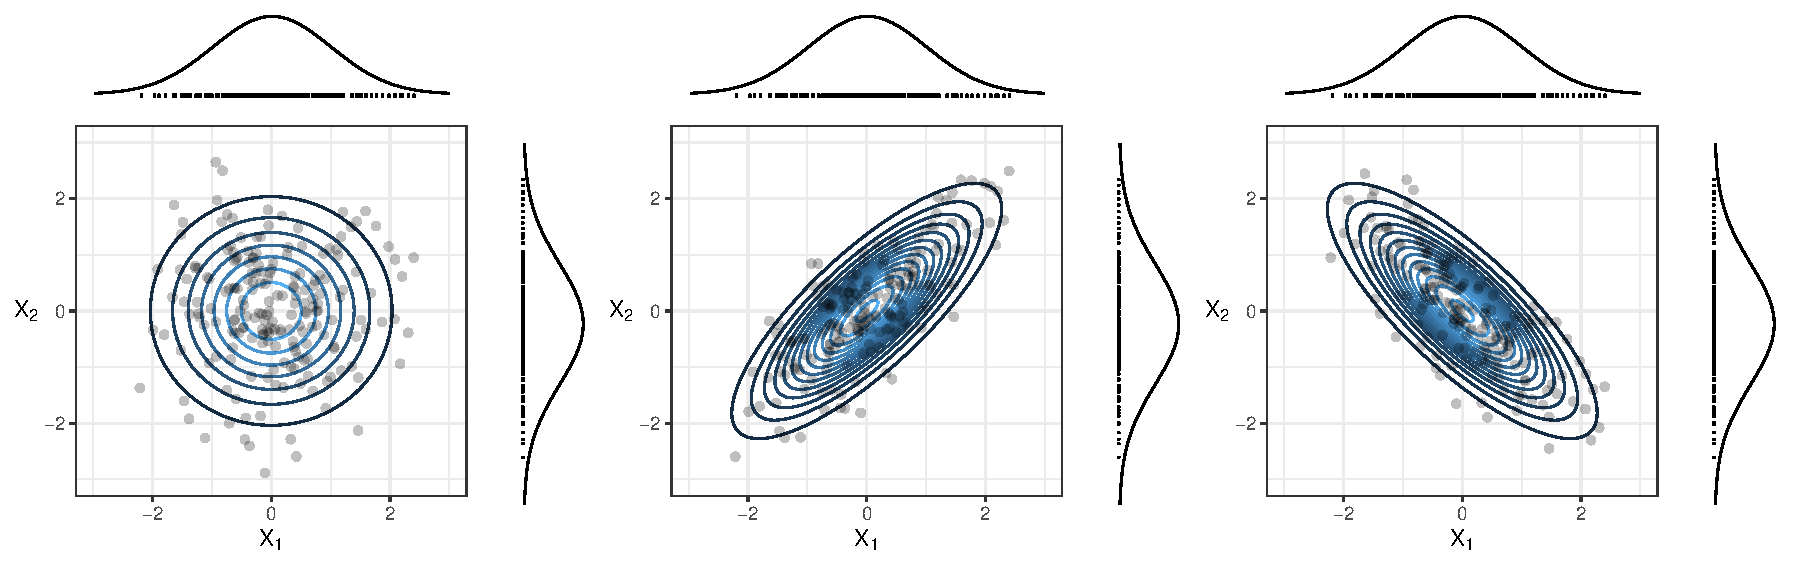
\includegraphics[width = 0.9\textwidth]{figure/dnorm_correlation.pdf}
\end{center}}

\only<2>{\begin{center}
\begin{minipage}[t]{0.2\textwidth}
\centering{\scriptsize
 $\rho(X_1, X_2) = 0$ \\(independent)}
\end{minipage}
\begin{minipage}[t]{0.2\textwidth}
\centering{\scriptsize
 $\rho(X_1, X_2) = 0.8$}
\end{minipage}
\begin{minipage}[t]{0.2\textwidth}
\centering{\scriptsize
 $\rho(X_1, X_2) = -0.8$}
\end{minipage}\\
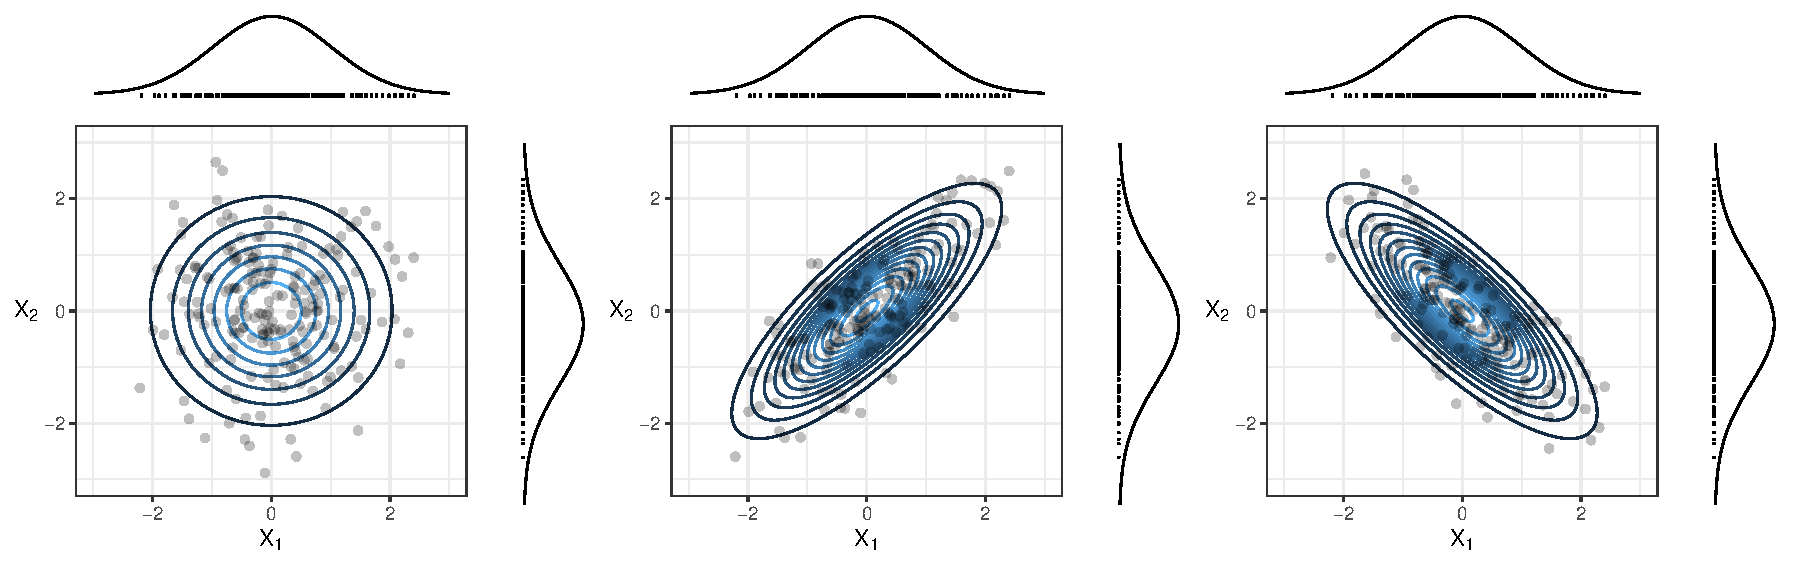
\includegraphics[width = 0.6\textwidth]{figure/dnorm_correlation.pdf}
\end{center}


Examples with Pearson's correlation $\rho \approx 0$ but non-linear dependencies (MI $\neq 0$):\\
\medskip
\centering
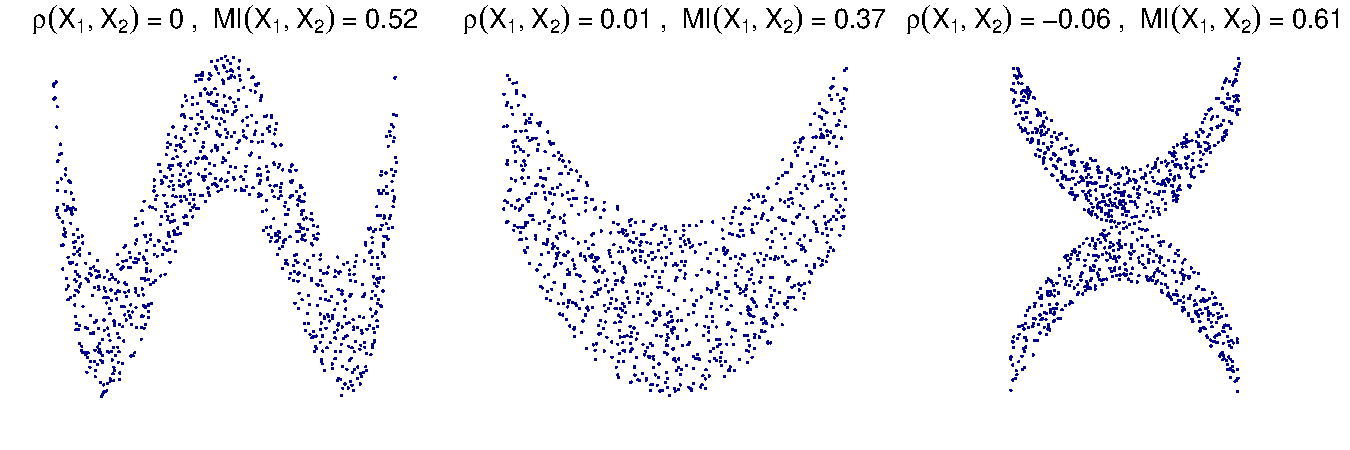
\includegraphics[width = 0.95\textwidth]{figure/dependence_3}}
\end{frame}


% \begin{frame}{Interpretations with Dependent Features}
% \begin{itemize}

% % \item Be clear about interpretation goal: Explain model or underlying relationship in data?
% % %We need to differentiate between interpretations of a model or reality
% % \\
% % $\leadsto$ Latter might be distorted by modeling fallacies, 
% % e.g., 
% % %due to bad data quality, 
% % under- and overfitting or extrapolation

% %\pause
% \item Highly correlated features contain similar information \\
% $\leadsto$ Model might pick only 1 feat. (regularization), even if it is causally irrelevant \\
% %Some models might use only one correlated feature (even if it is causally not relevant)
% %Can confuse a model so that only one correlated feature is used (even if it is not relevant) \\
% $\leadsto$ Produced explanations can be misleading (true to model, but not to data) % generating process
% \\
% $\leadsto$ E.g., different interpretable models produce different results
% %$\leadsto$ Different IML models often produce different results in these situation, and not always trivial to understand which / why 
% %Even for two causally and equally relevant correlated features it is not guaranteed that their explanations will be similar
% % \pause
% % \item Assume two causally and equally relevant but highly correlated features \\
% % $\leadsto$ One might expect that their explanations (e.g., feature importance) will be similar \\
% % %One might expect that explanations of two correlated features (e.g., feature importance) are similar as they share similar information \\
% % $\leadsto$ Generally not true as the model can learn different relationships


% % \begin{tikzpicture}[remember picture,overlay,shift=(current page.center)] %opacity=.2,text opacity=1
% % \node[fill=white, opacity=1,text opacity=1] at (current page.center) {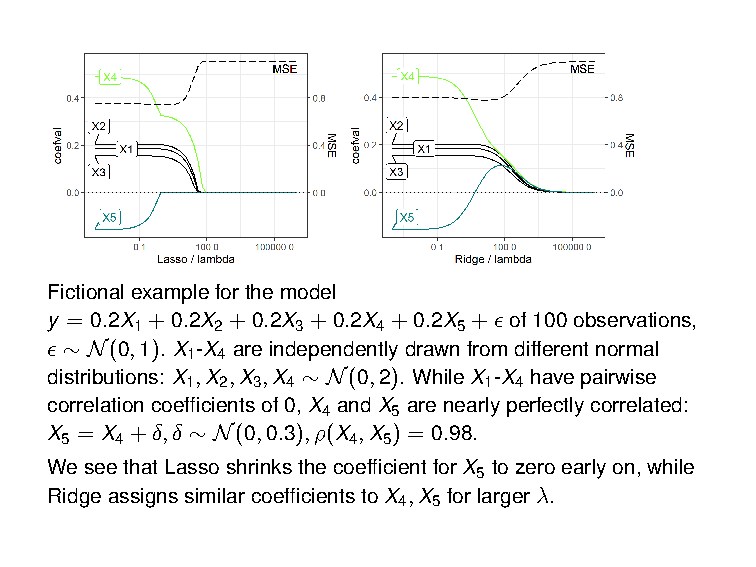
\includegraphics[width=0.6\textwidth]{figure/ridge_lasso}};
% % \end{tikzpicture}
% \pause

% % \only<3>{
% %  \begin{BlueBox}{Example}
% %   \begin{columns}[c, totalwidth=\textwidth]
% % \begin{column}{0.5\textwidth}
% % 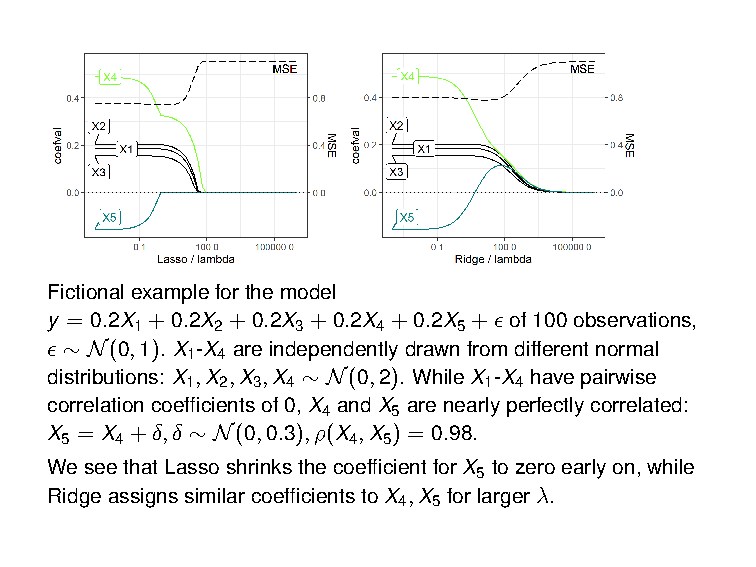
\includegraphics[trim=0px 110px 30px 0px, clip, width=\textwidth]{figure/ridge_lasso}
% % \end{column}
% % \begin{column}{0.5\textwidth}
% % 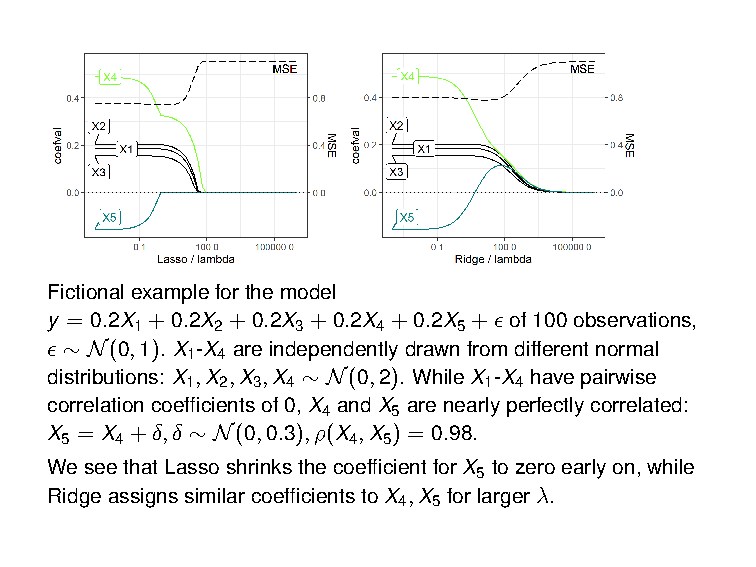
\includegraphics[trim=0px 0px 0px 115px, clip, width=\textwidth]{figure/ridge_lasso}
% % \end{column}
% % \end{columns}}
% % \end{BlueBox}
% % }

% %\only<3>{
% %\colorbox{blue!20}{
% %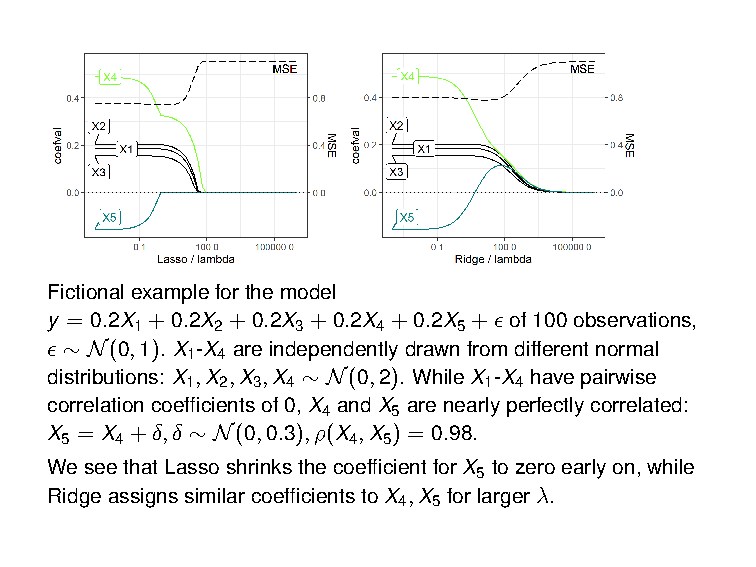
\includegraphics[trim=0px 0px 0px 115px, clip, width=.55\linewidth]{figure/ridge_lasso}}
% %\begin{columns}[T, totalwidth = \textwidth]
% %    \begin{column}{0.5\textwidth}
% %\scriptsize
% \item \textbf{Example:} Simulate 100 obs. from DGP $Y = 0.2 (X_1 + \dots + X_5) + \epsilon, \epsilon \sim N(0,1)$

% \centerline{%\colorbox{blue!20}{
% 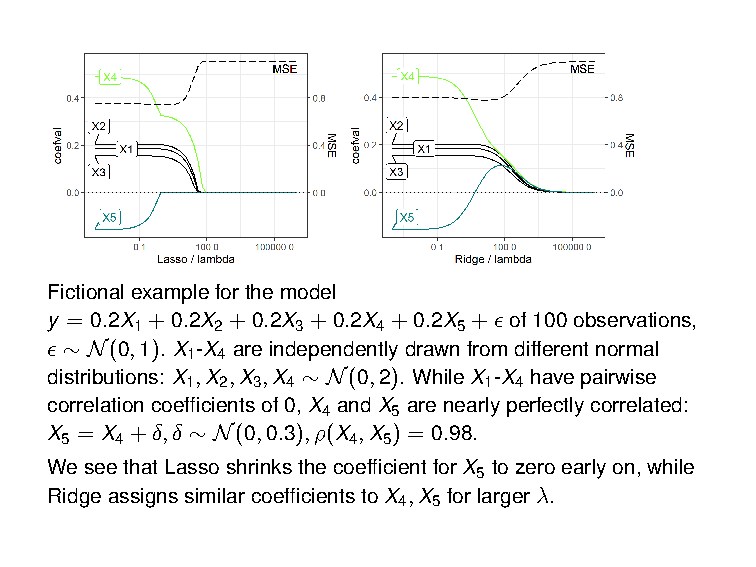
\includegraphics[trim=0px 110px 30px 0px, clip, width=0.8\textwidth]{figure/ridge_lasso} }%}
% %    \end{column}
% %    \begin{column}{0.5\textwidth}
        
% \begin{itemize}
%     \item $X_1, \dots, X_4 \sim N(0, 2)$ (uncorrelated)
%     \item $X_5 = X_4 + \delta, \delta \sim N(0, 0.3)$ $\Rightarrow \rho(X_4, X_5) = 0.98$ (highly correlated)
%     \item LASSO: Shrinks coef. of $X_5$ to zero, coef. of $X_4$ about $1.5 \times$ higher
%     \item Ridge: Similar coef. for $X_4$ and $X_5$ for higher lambda
% \end{itemize}
% %    \end{column}
% %\end{columns}

% \end{itemize}

% \end{frame}



% \begin{frame}{Extrapolation due to Dependencies}
% %\begin{center}
% \centerline{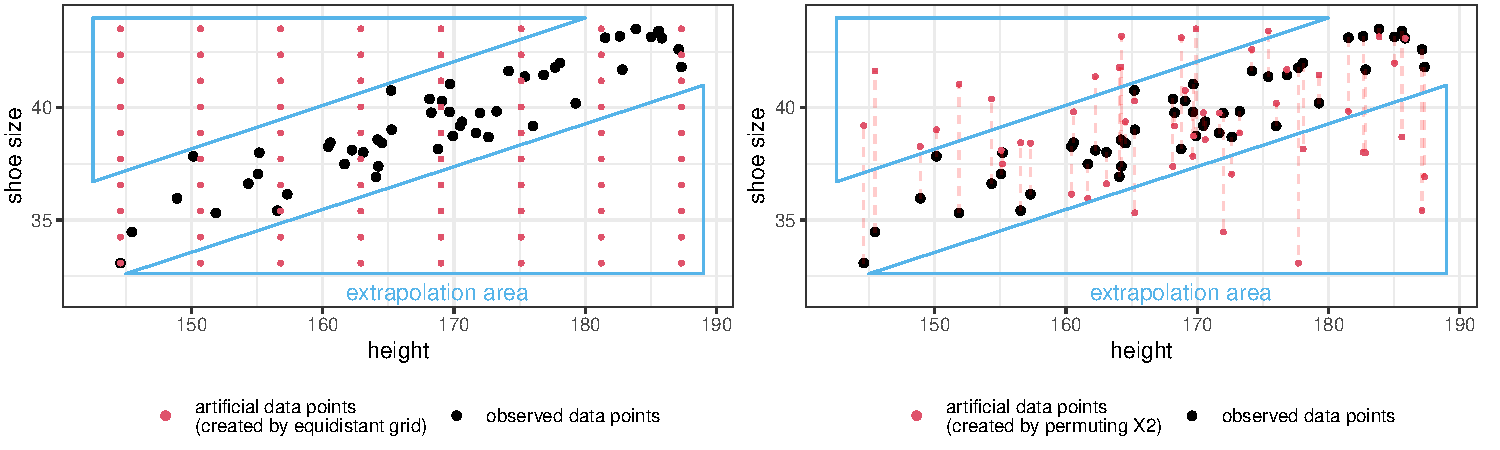
\includegraphics[width=\textwidth]{figure/extrapolation}}
% %\end{center}

% \begin{itemize}
% %\itemsep1em
% \item Many interpretation methods are based on
% %rely on varying feature values and create
% artificially created data points \\
% $\leadsto$ Many points lie in low-density regions if features are dependent\\
% $\leadsto$ Predictions in such regions have high uncertainty\\ % in regions with no or few training data
% $\leadsto$ Explanations can be biased if they rely on pred. where model extrapolated\\
% \pause
% %\item 
% %\item Essentially, we are interested in the prediction uncertainty\\
% %, i.e., the less the training data on a feature subspace, the higher the prediction uncertainty.
% %$\leadsto$ Models are rarely able to quantify uncertainty of predictions %Models are rarely capable of quantifying prediction uncertainty
% \item There is no definition of when a model extrapolates and to what degree \\
% $\leadsto$ Severity of extrapolation depends on model %, some extrapolate more than others 
% \\
% $\leadsto$ Density of train data may helps identify regions where extrapolation is likely \\
% \phantom{$\leadsto$} But: Density estimation in many dimensions is often infeasible
% %$\leadsto$ Some models might extrapolate more than others
% %\item Density of training data might serve as proxy to identify regions where extrapolation is likely\\
% %$\leadsto$ Density estimation in many dimensions is often infeasible
% \end{itemize}

% \end{frame}

%%% dann das gleiche für interactions

%% wir können auch ein bsp mit feature importannce machen, wo korrelation alles schwieriger macht. im guyon paper und im i2ml featsel teil ist es drin

%% was kann mindestens zu korrel sagen:
%
% a) das extrapol problem. haben wir folien zu
% b) bei korrel kann man sagen: die vars haben die gkleich info, also breaucht man nur eine. das ist eine explanation. die kann aber falsch sein. siehe guyon bsp
% c) bei korrel könnte man sagen: die erklärungen zu vars sind die gleichen. zb deren importance. das ist aber auch nicht gegeben
% ---> generell: vorsicht!

%--------------------------------

% bei interactions:
% 1) definition davon bringen
% man kann das operationals / an der modell struktur erklären. als bsp lin modell und tree
% allgemeine definition von fanoava
% sagen dass eine funktin keine IA hat, wenn sie separierbar. verbindung zur optimierung bringen
% sagen dass man aus der fanbova die interactioons ablesen kann und auf die H-statistic für weiteres vereweisen

\endlecture
\end{document}
